\section{Computation-Risk Tradeoffs for Dropout and Subsampling}
\label{sec:subsampling}

We begin by considering one of the simplest settings, where
the task is to fit a linear regression model according to the least squares
criterion
\begin{equation}
\hat \beta_n = \argmin_\beta \|\Y - \X\beta\|_2
\end{equation}
where $\Y$ is an $n$-vector of response variables, and $\X$ is an
$n\times p$ design matrix of predictor variables, formed from data
$(X_i, Y_i)$, with $X_i\in\reals^p$ and $Y_i\in\reals$, for
$i=1,\ldots, n$, with $n\gg p$.  Computing the least squares
estimator $\hat\beta_n = (\X^T \X)^{-1} \X^T \Y$ directly requires
$O(np^2 + p^3)$ computation, with the first term the computation
required to compute the sample covariance $\frac{1}{n} \X^T \X$,
and the second term the computation required to compute its inverse.
Assuming that the data are generated according to a linear model
$Y_i = X_i^T \beta^* + \epsilon_i$, with $\Var(\epsilon_i) =
\sigma^2$, standard analysis shows the squared error decays as
$\E(\|\hat\beta_n - \beta^*\|_2^2) = O(p/n)$.

The easiest way of making a computation-risk tradeoff is to simply 
subsample the data.  Suppose that $\X_m$ is a random sample
of $m$ rows of $\X$, with corresponding response $Y_m$.
Then the least squares estimator $\hat \beta_m =
(\X_m^T \X_m)^{-1} \X_m^T \Y_m$ 
has error scaling as $\|\hat\beta_m - \beta^*\|_2^2 = O(p/m)$
and computation scaling as $O(m p^2 + p^3)$.  

As an alternative, suppose that we dropout random entries from $\X$
rather than removing entire rows.  In particular, let
\begin{equation}
\Xdrop = \X \hadamard \bZ
\end{equation}
where $\bZ \sim \text{Bernoulli}(\theta)$ is an $n\times p$ matrix of
$\{0,1\}$ values $Z_{ij} \sim \text{Bernoulli}(\theta_j)$, and 
$\mbf{A}\hadamard \mbf{B}$ denotes the Hadamard (pointwise) product
of matrices $\mbf{A}$ and $\mbf{B}$.  We then compute the
estimator
\begin{equation}
\drop{\beta}_n = \argmin_\beta \|Y - \drop{\X} \beta\|_2 ^2.
\end{equation}

\vskip10pt
\centerline{\textit{\small BACKGROUND ON SUBSPACE EMBEDDING HERE}}
\vskip10pt

Using fast subspace embedding algorithms, the estimator
$\drop{\beta}_n$ can be computed in time
$O\bigl(\textit{nnz}(\drop{\X}) +p^3\bigr)$.
Since the mean number of nonzeros is $\E_\theta\bigl( \nnz{\drop{\X}}\bigr) =
\sum_{j=1}^p n\theta_j$, we can express this
computation time as $O_P\bigl( n\|\theta\|_1 + p^3\bigr)$
where the $O_P$ indicates that the bound holds with high probability.
The key question is, how does the risk scale, and do we obtain
a favorable tradeoff relative to subsampling?

Figure~\ref{fig:doss} shows the results of simulations comparing the
estimators based on subsampling and the dropout.  For the dropout
method, each data item $X_{ij}$ is kept with probability $\theta_0$,
and dropped out with probability $1-\theta_0$, controlling the 
computation-risk tradeoff.  The simulation measures
computation in terms of the theoretical bounds
for optimal subspace embedding and directly solving for the least squares
estimator on the subsampled data.

\begin{figure}
\begin{center}
\begin{tabular}{cc}
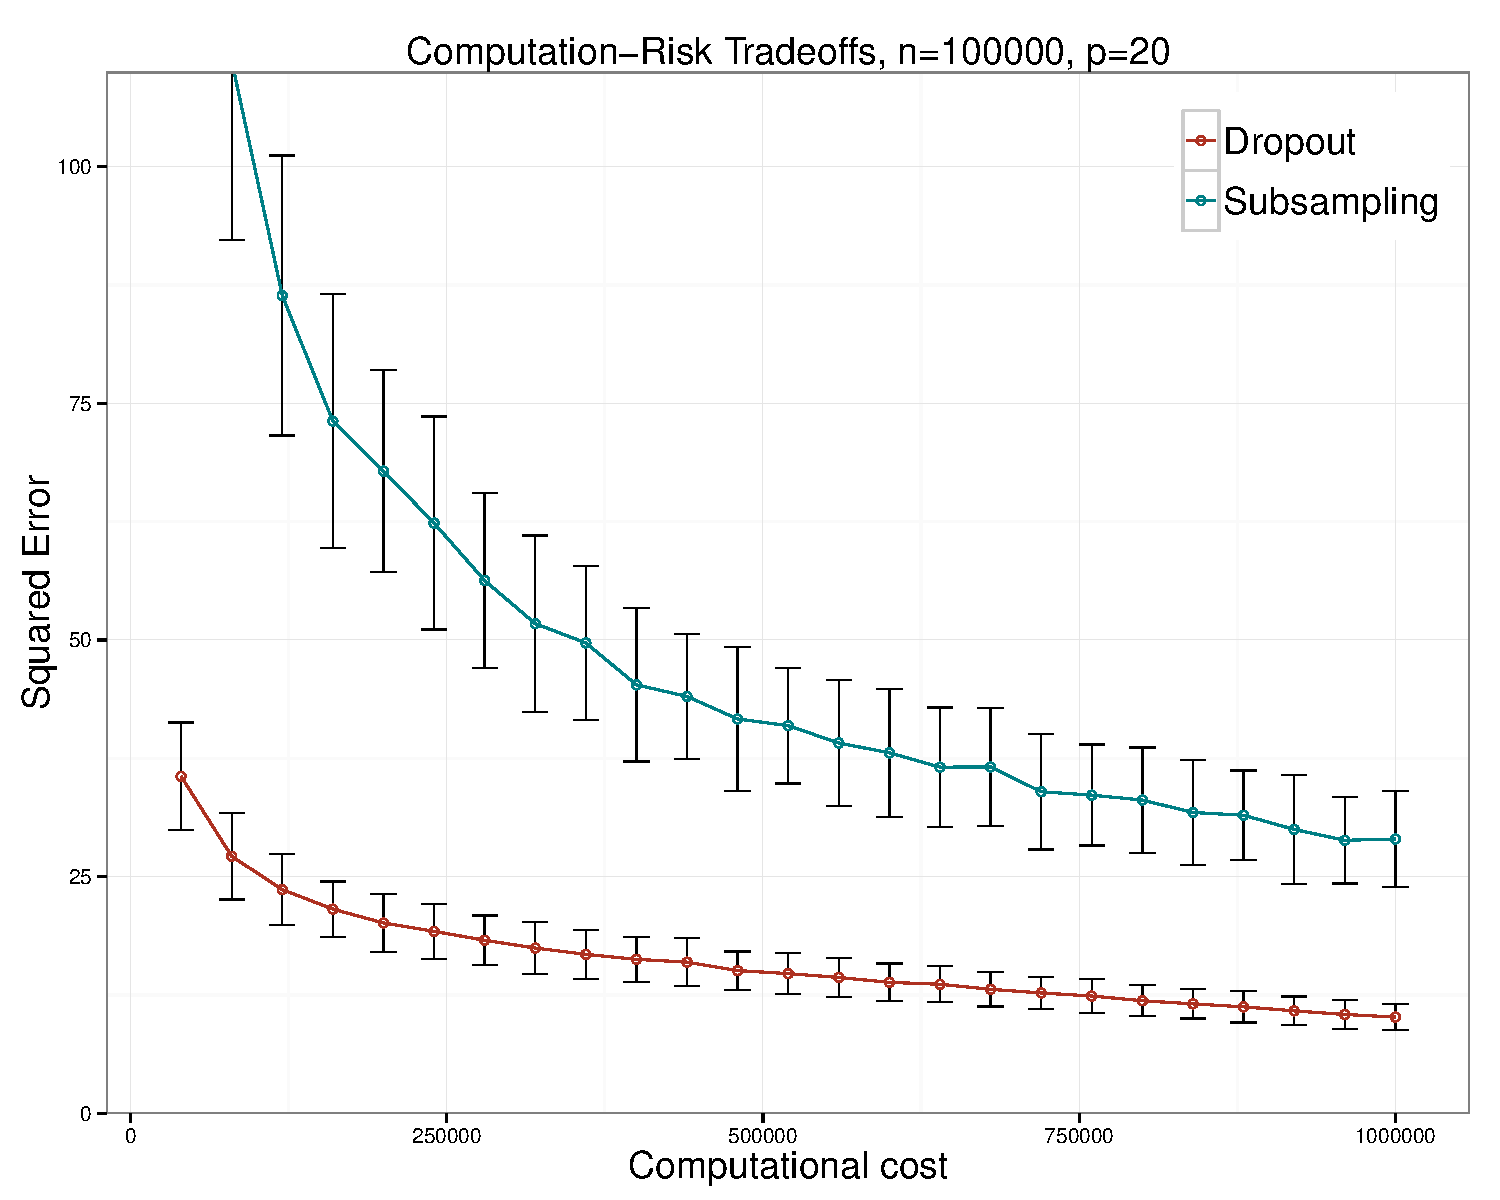
\includegraphics[width=.48\textwidth]{figs/dropout-subsample-n100000-p20-T100.pdf} &
\hskip-10pt
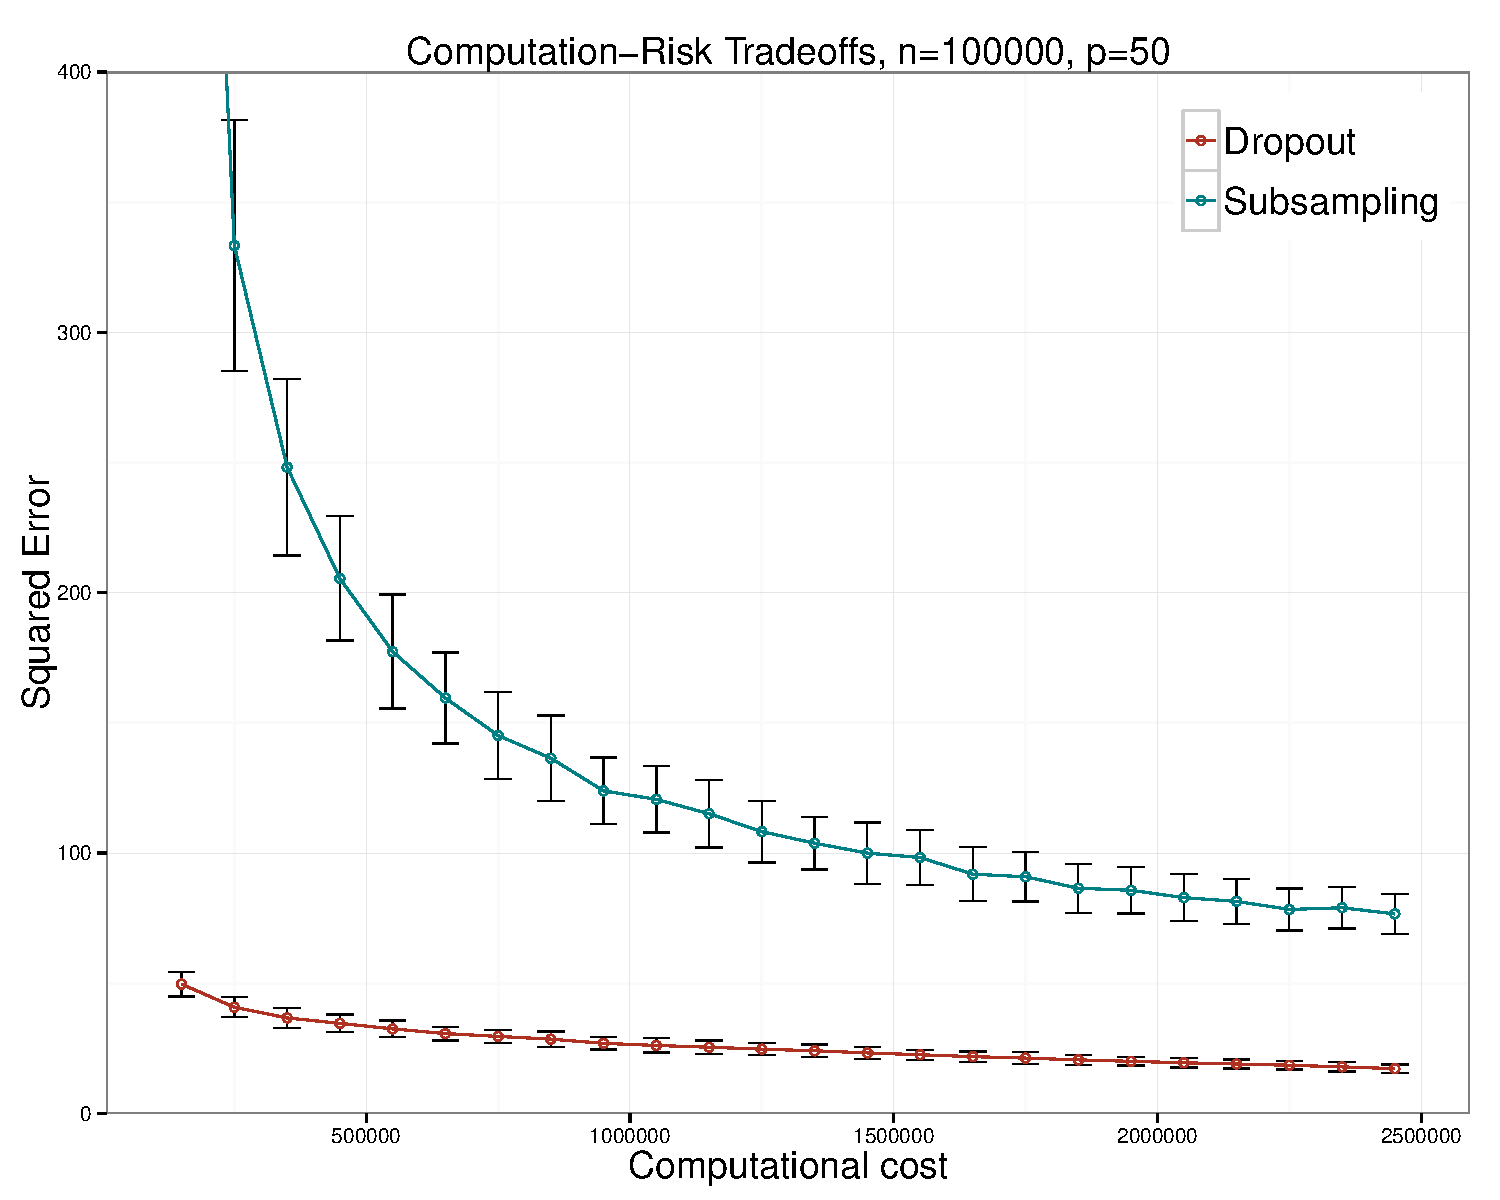
\includegraphics[width=.48\textwidth]{figs/dropout-subsample-n100000-p50-T100.pdf}
\end{tabular}
\end{center}
\caption{Comparision of subsampling to the dropout method for making
  computation-risk tradeoffs.  Two simulations are run, for $p=10$ and
  $p=20$ variables.  Subsampling with different subsample sizes $m$ is
  compared to the dropout with different dropout rates $\theta$.  The
  computational costs are measured by the theoretical bounds $O(mp^2 +
  p^3)$ for subsampling and $O(n\|\theta\|_1 + p^3)$ for the dropout,
  solved with subspace embedding. As $p$ increases, so does the
  relative advantage of the dropout.}
\label{fig:doss}
\end{figure}





